\documentclass{beamer}

% For more themes, color themes and font themes, see:
% http://deic.uab.es/~iblanes/beamer_gallery/index_by_theme.html
%
\mode<presentation>
{
  \usetheme{Darmstadt}       % or try default, Darmstadt, Warsaw, ...
  \usecolortheme{default} % or try albatross, beaver, crane, ...
  \usefonttheme{default}    % or try default, structurebold, ...
  \setbeamertemplate{navigation symbols}{}
  \setbeamertemplate{caption}[numbered]
} 

\usepackage[T1]{fontenc}
\usepackage[frenchb]{babel}
\usepackage[utf8x]{inputenc}
\usepackage{array}
\usepackage{booktabs}
\usepackage{adjustbox}

% On Overleaf, these lines give you sharper preview images.
% You might want to `comment them out before you export, though.
\usepackage{pgfpages}
\pgfpagesuselayout{resize to}[%
  physical paper width=8in, physical paper height=6in]

% Here's where the presentation starts, with the info for the title slide
\title{Appel d'offre PICASO}
\author{Nicolas Bonfante - Luc Forget - Quentin Labernia \\ Paul Compagnon - Marc Javin - Ghayth Baroumi}
\institute{INSA Lyon}
\date{\today}

\begin{document}

\begin{frame}
\begin{center}
\huge E-kitable
\end{center}
\maketitle
\end{frame}

% These three lines create an automatically generated table of contents.
\begin{frame}{Plan}
  \tableofcontents
\end{frame}

\section{Marketing}
% Marketing partie 1

\begin{frame}{Présentation du produit}
Concept de table en blocs
\begin{itemize}
\item 4 blocs
\begin{itemize}
\item Bloc standard
\item Bloc thermique
\item Bloc électrique
\item Bloc électrique thermique
\end{itemize}
\item Personnalisable à l'infini
\end{itemize}
\end{frame}

\begin{frame}{Utilisation}
\begin{itemize}
\item Utilisation diverse
\begin{itemize}
\item Dans une cuisine : blocs thermiques
\item Pour un bureau : bloc électrique et thermique
\end{itemize}
\end{itemize}
\end{frame}

\begin{frame}{Matériaux et qualité}
\begin{itemize}
\item Bois brut pour le plateau et les pieds
\item Petite quincaillerie pour le reste
\item Haute qualité
\end{itemize}
\end{frame}

\begin{frame}{Nature et délai de distribution}
\begin{itemize}
\item Nature de la distribution
\begin{itemize}
\item Grands magasins et magasins spécialisés
\item Vente en ligne via configurateur
\end{itemize}
\item Délai 
\begin{itemize}
\item 3 jours en magasins
\item 7 jours via internet
\begin{itemize}
\item 3 jours si souscription au service premium
\end{itemize}
\end{itemize}
\end{itemize}
\end{frame}
% Marketing partie 2
\begin{frame}{Quantité de distribution}
\begin{itemize}
\item<1-> Approvisionnement initial des distributeurs avec une quantité dépendant de leur rayonnement
\item<2-> Gestion des stocks de pièces de bases en kanban par les distributeurs
\item<3-> Contractualisation éventuelle d'un stock minimal présent chez le distributeur
\end{itemize}
\end{frame}

\begin{frame}{Localisation de la distribution}
	\begin{itemize}
		\item<1-> Format du meuble adapté à la distribution en grande surface (spécialisée en bricolage ou de grande distribution)
		\item<2-> Cible géographique : implantation initiale sur les marchés savoyards (localité) et parisiens (visibilité)
		\item<3-> Expansion progressive sur tout le marché français prévue sur 8 mois.
	\end{itemize}
\end{frame}

\begin{frame}{Prévisions de vente}
\adjustbox{max height=\dimexpr\textheight-5.5cm\relax,
           max width=\textwidth}{
	\begin{tabular}{>{\bfseries}r>{\centering\arraybackslash}m{0.27\textwidth}>{\centering\arraybackslash}m{0.27\textwidth}>{\centering\arraybackslash}m{0.27\textwidth}}
		\toprule
		& \textbf{Pied de table (x8)} & \textbf{Blocs standards (x24)} &
		\textbf{Blocs
		thermiques (x6)} \\
		\midrule
		Juin 16 & 30 & 27 & 12\\
		Juil. 16 & 90 & 81 & 36\\
		Août 16 & 210 & 219 & 88\\
		Sept.16 & 432 & 465 & 198 \\
		Oct. 16 & 765 & 800 & 402\\
		Nov. 16 & 1024 & 1200 & 580 \\
		Déc. 16 & 1148 & 1345 & 700 \\
		Janv. 17 & 1224 & 1445 & 732\\
		Fév. 17 & 900 & 1600 & 700\\
		Mars 17 & 800 & 1585 & 700\\
		Avril 17 & 750 & 1615 & 680\\
		Mai 17 & 800 & 1579 & 700\\
		\bottomrule
	\end{tabular}}
\end{frame}

\section{Méthode}
% Methode partie 1

\begin{frame}{La différenciation retardée}
\begin{itemize}
\item<1-> Blocs de 30*30 standards 
\item<2-> Pieds standards
\item<3-> Peinture / Lasure
\item<4-> Revêtement thermique
\item<5-> Trou 
\end{itemize}
\end{frame}

\begin{frame}{Nomenclature}
	\begin{figure}[H]
\centering
\includegraphics[scale=0.4]{../Methodes/captures/Bloc_base.png}
\caption{Nomenclature du bloc}
	\end{figure}		
\end{frame}

\begin{frame}{Nomenclature}
	\begin{figure}[H]
\centering
\includegraphics[scale=0.4]{../Methodes/captures/Pieds.png}
\caption{Nomenclature du pied}
	\end{figure}		
\end{frame}

\begin{frame}{Procédés}
	\begin{figure}[H]
\centering
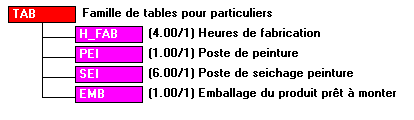
\includegraphics[scale=0.4]{../Methodes/captures/procede_fab_table_particulier.PNG}
\caption{Procédé}
	\end{figure}		
\end{frame}

% Methode partie 2

\begin{frame}{Adaptation des moyens de production}
	Au vu de l'organisation actuelle de l'entreprise,
	il est nécessaire d'effectuer les changements suivants :
	
	\begin{itemize}
		\item<1-> achat de deux machines de conditionnement,
		\item<2-> deux transpalettes électriques,
		\item<3-> d'une mélangeuse industrielle,
		\item<4-> mise en place d'un poste de travail muni d'une hotte.
	\end{itemize}
	
\end{frame}

\begin{frame}{Politiques d'approvisionnement et de production}
	Une politique d'approvisionnement privilégiée :
	\begin{itemize}
		\item<1-> gestion sur consommation principalement,
		\item<2-> gestion sur besoin pour les teintes de peinture
		et de lasures peu demandées.
	\end{itemize}
	\begin{center}
		\item<3->{Planification de la production via MRP1}
	\end{center}
\end{frame}

\begin{frame}{Production}
	Les flux de production prévus :
	\begin{itemize}
	\item<1-> fabrication des articles standards par production en ligne,
	\item<2-> production par lot des articles en différentiation retardée.
	\end{itemize}
\end{frame}



\section{Organisationnel}
% Orga partie 1
% Orga partie 2

\section{Conlusion}
\begin{frame}
\begin{center}
Merci pour votre attention ! \\
\vspace{1cm}
Thank you for you attention ! \\
\vspace{1cm}
Danke für Ihre Aufmerksamkeit ! \\
\vspace{1cm}
¡ Gracias por su atención ! \\
\end{center}
\end{frame}


\end{document}